\documentclass[12pt, titlepage]{article}

\usepackage{fullpage}
\usepackage[round]{natbib}
\usepackage{multirow}
\usepackage{booktabs}
\usepackage{tabularx}
\usepackage{graphicx}
\usepackage{float}
\usepackage{hyperref}
\usepackage{indentfirst}
\hypersetup{
    colorlinks,
    citecolor=black,
    filecolor=black,
    linkcolor=red,
    urlcolor=blue
}
\usepackage[round]{natbib}

\newcounter{acnum}
\newcommand{\actheacnum}{AC\theacnum}
\newcommand{\acref}[1]{AC\ref{#1}}

\newcounter{ucnum}
\newcommand{\uctheucnum}{UC\theucnum}
\newcommand{\uref}[1]{UC\ref{#1}}

\newcounter{mnum}
\newcommand{\mthemnum}{M\themnum}
\newcommand{\mref}[1]{M\ref{#1}}

\title{SE 3XA3: Module Guide\\DNA Says}

\author{Team \#10, Team Name: DNA
		\\ Kareem Abdel Mesih - abdelk2
		\\ John-Paul Dakran - dakranj
		\\ Shady Nessim - nessimss
}

\date{\today}

\begin{document}

\maketitle

\pagenumbering{roman}
\tableofcontents
\listoftables
\listoffigures

\begin{table}[H]
\caption{\bf Revision History}
\begin{tabularx}{\textwidth}{p{3cm}p{2cm}X}
\toprule {\bf Date} & {\bf Version} & {\bf Notes}\\
\midrule
3/11/2016 & 1.0 & Addition of section 2\\
7/11/2016 & 1.1 & Addition of section 3\\
8/11/2016 & 1.2 & Addition of section 1\\
11/11/2016 & 1.3 & Addition of section 4\\
\bottomrule
\end{tabularx}
\end{table}

\newpage

\pagenumbering{arabic}

\section{Introduction}

\subsection{Overview}
\par This project is a redevelopment of the famous game Simon Says, with a slight modification that makes DNA Says unique while keeping the integrity of the game consistent with the original version. The game consists of three distinct modes - Kareem Says, JP Says and Shady Says.

\subsection{Context}
\par This document consists of the Module Guide (MG) for the project DNA Says. This is the second portion of the design documentation along with the Module Interface Specification (MIS) - which explains the semantics of the code in natural language. \\
\par The Module Guide is a decomposition of the software system into modules. A module is an independent self-contained unit that makes up a complex software system. Decomposing a problem into modules is an extremely important aspect of software design as it promotes the principle of information hiding. Each module is completed concurrently by a programmer and houses a secret of the modules functionality.\\
\par The Module Guide (MG) reveals how the software system will carry out the functionality that is described in the Software Requirements Specification (SRS) document. The potential readers of the document are listed below:
\begin{itemize}
\item Designers/Developers: This document is extremely important for the designers of the software system. It provides a means for the designers to easily identify different parts of the software and relate the implementation to the requirements.
\item New Project Members: This document allows new project members to easily identify the components of the software system. It is a simple way to understand and locate information that relates to specific parts of the software. 
\item Maintainers: The hierarchical structure of the module guide improves the maintainers' understanding when they need to make changes to the system. It is important for a maintainer to update the relevant sections of the document after changes have been made.
\end{itemize}

\subsection{Design Principles}
\par The first major design principle utilized by the developers of DNA Says is modularity. This design principle was achieved by dividing the software into independent self-contained units. After the conncurrent development of the individual modules they are integrated together to full the functional and non-functional requirements in the SRS.\\

\par The second major design principle used in this software system is abstraction. After division of the software system into modules, each module was viewed at an abstract level. In other words, the design team neglected the implementation of the module and focused on the most essential information which is relevant to that specific module.  \\

\par The third major design principle utilized by the developers of DNA Says is information hiding. This design principle was employed during the development of the individual modules. The theory behind this principle is that the modules were designed in such a way that the information and secret of a module cannot be exposed to other modules that do not need to know that information.



\subsection{Document Structure}


The rest of the document is organized as follows. Section
\ref{SecChange} lists the anticipated and unlikely changes of the software
requirements. Section \ref{SecMH} summarizes the module decomposition that
was constructed according to the likely changes. Section \ref{SecConnection}
specifies the connections between the software requirements and the
modules. Section \ref{SecMD} gives a detailed description of the
modules. Section \ref{SecTM} includes two traceability matrices. One checks
the completeness of the design against the requirements provided in the SRS. The
other shows the relation between anticipated changes and the modules. Section
\ref{SecUse} describes the use relation between modules.

\subsection{Naming Conventions \& Terminology}

\begin{table}[hbp]
\caption{\textbf{Table of Abbreviations}} \label{Table}
\begin{tabularx}{\textwidth}{p{3cm}X}
\toprule
\textbf{Abbreviation} & \textbf{Definition} \\
\midrule
MG & Module Guide\\
SRS & Software Requirements Specification\\
MVC & Model View Controller\\
\bottomrule
\end{tabularx}
\end{table}


\begin{table}[!htbp]
\caption{\textbf{Table of Definitions}} \label{Table}
\begin{tabularx}{\textwidth}{p{3cm}X}
\toprule
\textbf{Term} & \textbf{Definition}\\
\midrule
Mode & Different subsections of the game\\
Gantt Chart & Chart outlining the timeline of the project\\
Python & A programming language\\
Pygame & Cross-platform set of Python modules designed for writing video games\\
\bottomrule
\end{tabularx}
\end{table}	


\section{Anticipated and Unlikely Changes} \label{SecChange}

This section lists possible changes to the system. According to the likeliness
of the change, the possible changes are classified into two
categories. Anticipated changes are listed in Section \ref{SecAchange}, and
unlikely changes are listed in Section \ref{SecUchange}.

\subsection{Anticipated Changes} \label{SecAchange}

Anticipated changes are the source of the information that is to be hidden
inside the modules. Ideally, changing one of the anticipated changes will only
require changing the one module that hides the associated decision. The approach
adapted here is called design for
change.

\begin{description}
\item[\refstepcounter{acnum} \actheacnum \label{acExecutable}:] The routine that the user follows to start the program. There will be an attempt to create a standalone application rather than require the user to install Python and Pygame.
\item[\refstepcounter{acnum} \actheacnum \label{acI1}:] The main menu.
\item[\refstepcounter{acnum} \actheacnum \label{acI2}:] The flow of the program. There will be a button within each mode to go back to the main menu.
\item[\refstepcounter{acnum} \actheacnum \label{acI3}:] The colours of labels and buttons of the main menu along with all the modes.
\item[\refstepcounter{acnum} \actheacnum \label{acI4}:] The size of the text in each mode.
\end{description}

\subsection{Unlikely Changes} \label{SecUchange}

The module design should be as general as possible. However, a general system is
more complex. Sometimes this complexity is not necessary. Fixing some design
decisions at the system architecture stage can simplify the software design. If
these decision should later need to be changed, then many parts of the design
will potentially need to be modified. Hence, it is not intended that these
decisions will be changed.

\begin{description}
\item[\refstepcounter{ucnum} \uctheucnum \label{ucIO}:] The MVC structure will be transformed to accommodate for the separation of concerns, along with information hiding.
\end{description}

\section{Module Hierarchy} \label{SecMH}

This section provides an overview of the module design. Modules are summarized
in a hierarchy decomposed by secrets in Table \ref{TblMH}. The modules listed
below, which are leaves in the hierarchy tree, are the modules that will
actually be implemented.

\begin{description}
\item [\refstepcounter{mnum} \mthemnum \label{mHH1}:] Hardware-Hiding Module*
\item [\refstepcounter{mnum} \mthemnum \label{mHH2}:] Main Module
\item [\refstepcounter{mnum} \mthemnum \label{mHH3}:] Menu Module
\item [\refstepcounter{mnum} \mthemnum \label{mHH4}:] JP Module
\item [\refstepcounter{mnum} \mthemnum \label{mHH5}:] Kareem Module 
\item [\refstepcounter{mnum} \mthemnum \label{mHH6}:] Shady Module
\item [\refstepcounter{mnum} \mthemnum \label{mHH7}:] Setup Module
\item [\refstepcounter{mnum} \mthemnum \label{mHH8}:] Update Module
\item [\refstepcounter{mnum} \mthemnum \label{mHH9}:] ShowInst Module
\item [\refstepcounter{mnum} \mthemnum \label{mHH10}:] ShowScore Module
\item [\refstepcounter{mnum} \mthemnum \label{mHH11}:] ShowGoBack Module
\item [\refstepcounter{mnum} \mthemnum \label{mHH12}:] DrawKeys Module
\item [\refstepcounter{mnum} \mthemnum \label{mHH13}:] FlashKeyAnimation Module
\item [\refstepcounter{mnum} \mthemnum \label{mHH14}:] ChangeBackgroundAnimation Module
\item [\refstepcounter{mnum} \mthemnum \label{mHH15}:] GameOverAnimation Module
\item [\refstepcounter{mnum} \mthemnum \label{mHH16}:] CheckForQuit Module



\end{description}


\begin{table}[H]
\centering
\begin{tabular}{p{0.3\textwidth} p{0.6\textwidth}}
\toprule
\textbf{Level 1} & \textbf{Level 2}\\
\midrule

{Hardware-Hiding Module} & ~ \\
\midrule

\multirow{7}{0.3\textwidth}{Behaviour-Hiding Module} 
& M3\\
& M7\\
& M8\\
& M9\\
& M10\\
& M11\\ 
& M12\\
\midrule

\multirow{3}{0.3\textwidth}{Software Decision Module} 
& M2\\
& M4\\
& M5\\
& M6\\
& M13\\
& M14\\
& M15\\
& M16\\

\bottomrule

\end{tabular}
\caption{Module Hierarchy}
\label{TblMH}
\end{table}
\textbf{Note*:} The Hardware-Hiding Module is not implemented in the hierarchy as there is no hardware involved in this software system.

\section{Connection Between Requirements and Design} \label{SecConnection}

\par When designing the software system DNA Says, one of the main priorities was satisfying all functional and non-function requirements outlined in the SRS. These functionalities are truly the essence of the game and the design should support each and every one of them. Each module outlined in Section \ref{SecMH} serves an underlying purpose of satisfying the functions of the software. For example, functional requirement \#11 states: 

\begin{center} \textbf{There will be a score icon in the bottom right corner.} \end{center}

Module \#10: ShowScore, is intended to serve the function of displaying the score in the bottom right corner. This module was designed in a specific way to support the functionality of requirement \#11. The connection between the full list of requirements and modules is listed in Table \ref{TblRT}.

\section{Module Decomposition} \label{SecMD}

Modules are decomposed according to the principle of ``information hiding''
proposed by \citet{ParnasEtAl1984}. The \emph{Secrets} field in a module
decomposition is a brief statement of the design decision hidden by the
module. The \emph{Services} field specifies \emph{what} the module will do
without documenting \emph{how} to do it. For each module, a suggestion for the
implementing software is given under the \emph{Implemented By} title. If the
entry is \emph{OS}, this means that the module is provided by the operating
system or by standard programming language libraries.

\subsection{Hardware Hiding Module (\mref{mHH1})}
\begin{description}
\item[Secrets:]The data structure and algorithm used to implement the virtual
  hardware.
\item[Services:]Serves as a virtual hardware used by the rest of the
  system. This module provides the interface between the hardware and the
  software. So, the system can use it to display outputs or to accept inputs.
\item[Implemented By:] OS
\end{description}

\subsection{Behaviour-Hiding Module}
\begin{description}
\item[Secrets:]The contents of the required behaviours.
\item[Services:]Includes programs that provide externally visible behaviour of
  the system as specified in the software requirements specification (SRS)
  documents. This module serves as a communication layer between the
  hardware-hiding module and the software decision module. The programs in this
  module will need to change if there are changes in the SRS.
\item[Implemented By:] N/A
\end{description}

\subsubsection{Menu Module (\mref{mHH3})}
\begin{description}
\item[Secrets:]Structure to display title, instructions, buttons. 
\item[Services:]Displays the main menu.
\item[Implemented By:] DNA Says
\end{description}

\subsubsection{Setup Module (\mref{mHH7})}
\begin{description}
\item[Secrets:]The format and implementation of the displaying surface.
\item[Services:]Sets up the displaying surface. Creates a window of a set width and height, and labels it. All graphics can then be displayed on that window.
\item[Implemented By:] DNA Says
\end{description}

\subsubsection{Update Module (\mref{mHH8})}
\begin{description}
\item[Secrets:]The structure of the refreshing of the display.
\item[Services:]Updates the display.
\item[Implemented By:] DNA Says
\end{description}

\subsubsection{ShowInst Module (\mref{mHH9})}
\begin{description}
\item[Secrets:]The format of the instructions.
\item[Services:]Displays the instructions.
\item[Implemented By:] DNA Says
\end{description}

\subsubsection{ShowScore Module (\mref{mHH10})}
\begin{description}
\item[Secrets:]The data structure that holds the score.
\item[Services:]Displays the score.
\item[Implemented By:] DNA Says
\end{description}

\subsubsection{ShowGoBack Module (\mref{mHH11})}
\begin{description}
\item[Secrets:]The structure behind the main menu button.
\item[Services:]Displays the main menu button text.
\item[Implemented By:] DNA Says
\end{description}

\subsubsection{DrawKeys Module (\mref{mHH12})}
\begin{description}
\item[Secrets:]The algorithm used to draw the buttons depending on the mode.
\item[Services:]Draws the buttons on the screen.
\item[Implemented By:] DNA Says
\end{description}


\subsection{Software Decision Module}
\begin{description}
\item[Secrets:] The design decision based on mathematical theorems, physical
  facts, or programming considerations. The secrets of this module are
  \emph{not} described in the SRS.
\item[Services:] Includes data structure and algorithms used in the system that
  do not provide direct interaction with the user. 
  % Changes in these modules are more likely to be motivated by a desire to
  % improve performance than by externally imposed changes.
\item[Implemented By:] N/A
\end{description}

\subsubsection{Main Module (\mref{mHH2})}
\begin{description}
\item[Secrets:]The algorithm used to initialize clock, sounds, fonts, and buttons.
\item[Services:]Initializes Pygame along with Pygame's clock, all required font sizes, the required sounds, and the main menu button in its set position. This function then proceeds to call the main menu function.
\item[Implemented By:] DNA Says
\end{description}

\subsubsection{JP Module (\mref{mHH4})}
\begin{description}
\item[Secrets:]The size of keys and their positions, the implementation of the display. The algorithm and implementation of the song pattern, both visual and auditory.
\item[Services:]Starts the mode JP Says with nine buttons in square form. It plays the elements that are contained in the pattern, then checks for the user's input. If the user clicked the correct button then its sound is played and its key is highlighted temporarily, and the score is incremented. In the meantime, the program appends a random element to the pattern to be played, and the pattern is played, and the cycle goes on. However, if the user clicks on the wrong key, the game will be over. The game will also end if the user clicks on one correct key, and waits for more than four seconds, assuming that there is more than one element in the last pattern played. If the user clicks on the main menu button, the program will redirect them to the main menu.
\item[Implemented By:] DNA Says
\end{description}

\subsubsection{Kareem Module (\mref{mHH5})}
\begin{description}
\item[Secrets:]The size of keys and their positions, the implementation of the display. The algorithm and implementation of the song pattern, both visual and auditory.
\item[Services:]Starts the mode Kareem Says with piano keyboard. It plays the elements that are contained in the pattern, then checks for the user's input. If the user clicked the correct button then its sound is played and its key is highlighted temporarily, and the score is incremented. In the meantime, the program appends a random element to the pattern to be played, and the pattern is played, and the cycle goes on. However, if the user clicks on the wrong key, the game will be over. The game will also end if the user clicks on one correct key, and waits for more than four seconds, assuming that there is more than one element in the last pattern played. If the user clicks on the main menu button, the program will redirect them to the main menu.
\item[Implemented By:] DNA Says
\end{description}

\subsubsection{Shady Module (\mref{mHH6})}
\begin{description}
\item[Secrets:]The size of keys and their positions, the implementation of the display. The algorithm and implementation of the song pattern, both visual and auditory.
\item[Services:]Starts the mode Shady Says with four buttons in square shape. It plays the elements that are contained in the pattern, then checks for the user's input. If the user clicked the correct button then its sound is played and its key is highlighted temporarily, and the score is incremented. In the meantime, the program appends a random element to the pattern to be played, and the pattern is played, and the cycle goes on. However, if the user clicks on the wrong key, the game will be over. The game will also end if the user clicks on one correct key, and waits for more than four seconds, assuming that there is more than one element in the last pattern played. If the user clicks on the main menu button, the program will redirect them to the main menu.
\item[Implemented By:] DNA Says
\end{description}

\subsubsection{FlashKeyAnimation Module (\mref{mHH13})}
\begin{description}
\item[Secrets:]The logic for playing patterns and flashing keys depending on mode.
\item[Services:]Plays the appropriate sound and flashes the correct key. For Kareem Says, it loads the correct note, and all highlights in this mode are bright red. The color of the keys is either white or black. For JP Says, it again loads the correct note and also each button is colored differently. For Shady Says, the sound is randomized every time and is stored in that sound variable.
\item[Implemented By:] DNA Says
\end{description}

\subsubsection{ChangeBackgroundAnimation Module (\mref{mHH14})}
\begin{description}
\item[Secrets:]The random RGB creation, the implementation of temporary display surface, the fading technique of colors.
\item[Services:]Changes the background color smoothly.
\item[Implemented By:] DNA Says
\end{description}

\subsubsection{GameOverAnimation Module (\mref{mHH15})}
\begin{description}
\item[Secrets:]The structure of changing background color and implementation of chord played.
\item[Services:]Plays the animation associated with incorrect user input. It plays a C chord while flashing the screen three times to indicate that the game is over.
\item[Implemented By:] DNA Says
\end{description}

\subsubsection{CheckForQuit Module (\mref{mHH16})}
\begin{description}
\item[Secrets:]The logic to detect quit request.
\item[Services:]Checks for quit requests. Quits the program at anytime upon the user's request.
\item[Implemented By:] DNA Says
\end{description}



\section{Traceability Matrix} \label{SecTM}

This section shows two traceability matrices: between the modules and the
requirements and between the modules and the anticipated changes.

% the table should use mref, the requirements should be named, use something
% like fref
\begin{table}[H]
\centering
\begin{tabular}{p{0.2\textwidth} p{0.6\textwidth}}
\toprule
\textbf{Req.} & \textbf{Modules}\\
\midrule
R1 & \mref{mHH}, \mref{mInput}, \mref{mParams}, \mref{mControl}\\
R2 & \mref{mInput}, \mref{mParams}\\
R3 & \mref{mVerify}\\
R4 & \mref{mOutput}, \mref{mControl}\\
R5 & \mref{mOutput}, \mref{mODEs}, \mref{mControl}, \mref{mSeqDS}, \mref{mSolver}, \mref{mPlot}\\
R6 & \mref{mOutput}, \mref{mODEs}, \mref{mControl}, \mref{mSeqDS}, \mref{mSolver}, \mref{mPlot}\\
R7 & \mref{mOutput}, \mref{mEnergy}, \mref{mControl}, \mref{mSeqDS}, \mref{mPlot}\\
R8 & \mref{mOutput}, \mref{mEnergy}, \mref{mControl}, \mref{mSeqDS}, \mref{mPlot}\\
R9 & \mref{mVerifyOut}\\
R10 & \mref{mOutput}, \mref{mODEs}, \mref{mControl}\\
R11 & \mref{mOutput}, \mref{mODEs}, \mref{mEnergy}, \mref{mControl}\\
\bottomrule
\end{tabular}
\caption{Trace Between Requirements and Modules}
\label{TblRT}
\end{table}

\begin{table}[H]
\centering
\begin{tabular}{p{0.2\textwidth} p{0.6\textwidth}}
\toprule
\textbf{AC} & \textbf{Modules}\\
\midrule
\acref{acHardware} & \mref{mHH}\\
\acref{acInput} & \mref{mInput}\\
\acref{acParams} & \mref{mParams}\\
\acref{acVerify} & \mref{mVerify}\\
\acref{acOutput} & \mref{mOutput}\\
\acref{acVerifyOut} & \mref{mVerifyOut}\\
\acref{acODEs} & \mref{mODEs}\\
\acref{acEnergy} & \mref{mEnergy}\\
\acref{acControl} & \mref{mControl}\\
\acref{acSeqDS} & \mref{mSeqDS}\\
\acref{acSolver} & \mref{mSolver}\\
\acref{acPlot} & \mref{mPlot}\\
\bottomrule
\end{tabular}
\caption{Trace Between Anticipated Changes and Modules}
\label{TblACT}
\end{table}

\section{Use Hierarchy Between Modules} \label{SecUse}

In this section, the uses hierarchy between modules is
provided. \citet{Parnas1978} said of two programs A and B that A {\em uses} B if
correct execution of B may be necessary for A to complete the task described in
its specification. That is, A {\em uses} B if there exist situations in which
the correct functioning of A depends upon the availability of a correct
implementation of B.  Figure \ref{FigUH} illustrates the use relation between
the modules. It can be seen that the graph is a directed acyclic graph
(DAG). Each level of the hierarchy offers a testable and usable subset of the
system, and modules in the higher level of the hierarchy are essentially simpler
because they use modules from the lower levels.

\begin{figure}[H]
\centering
%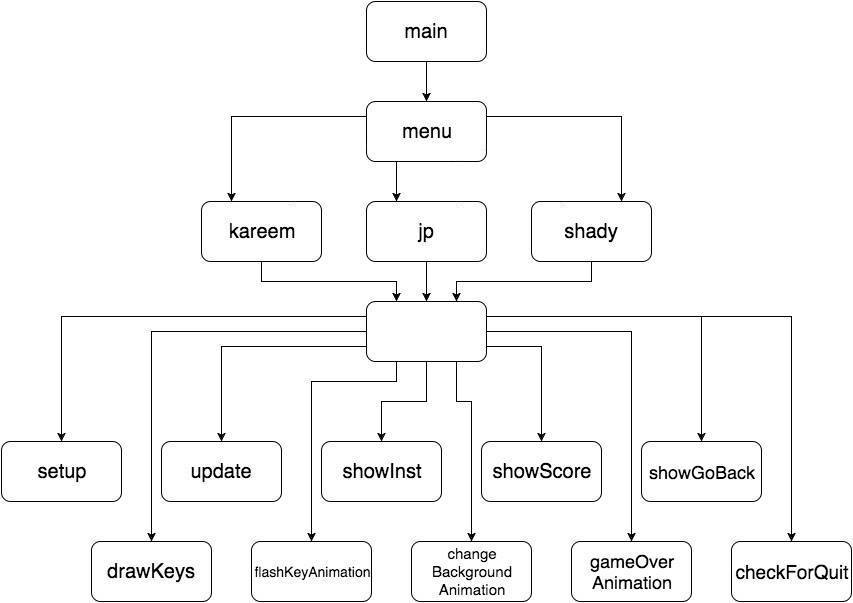
\includegraphics[width=0.7\textwidth]{UsesHierarchy.png}
\caption{Use hierarchy among modules}
\label{FigUH}
\end{figure}

%\section*{References}

\bibliographystyle {plainnat}
\bibliography {MG}

\end{document}